\section{Introduction}
	\noindent DRFM systems digitize and store incoming RF input signals at specific frequencies and bandwidths. The captured signals undergo time delays, frequency shifts and amplitude scalings, after which they are retransmitted. DRFM is used in order to synthesize false targets for radar systems by exploiting the radar assumptions of target identification. This is achieved by retransmitting a time delayed, amplitude scaled and frequency shifted coherent replica of the inputted signal, thereby making it, from the radar's perspective, indistinguishable from other genuine signals\cite{SJROOME}.\\ \newline  {\color{red} Radar Signal model} A DRFM system 	\\ \newline An illustration of a DRFM system may be seen in Fig.~\ref{fig:DRFM_Intro}. It can be seen that the input signal is mixed down to intermediate frequency and then is sampled by an Analog to Digital Converter (ADC). The sample rate of the ADC is equal to the bandwidth of the incoming RF signal as the ADC is sampling complex I/Q data. The digitized signal is then stored in memory and may be manipulated by means of the control interface. It must be noted that the memory is required to be The control interface is used to designate the various time delays, frequency shifts and amplitude scalings. 

	\begin{figure}[h!]
		\centering
		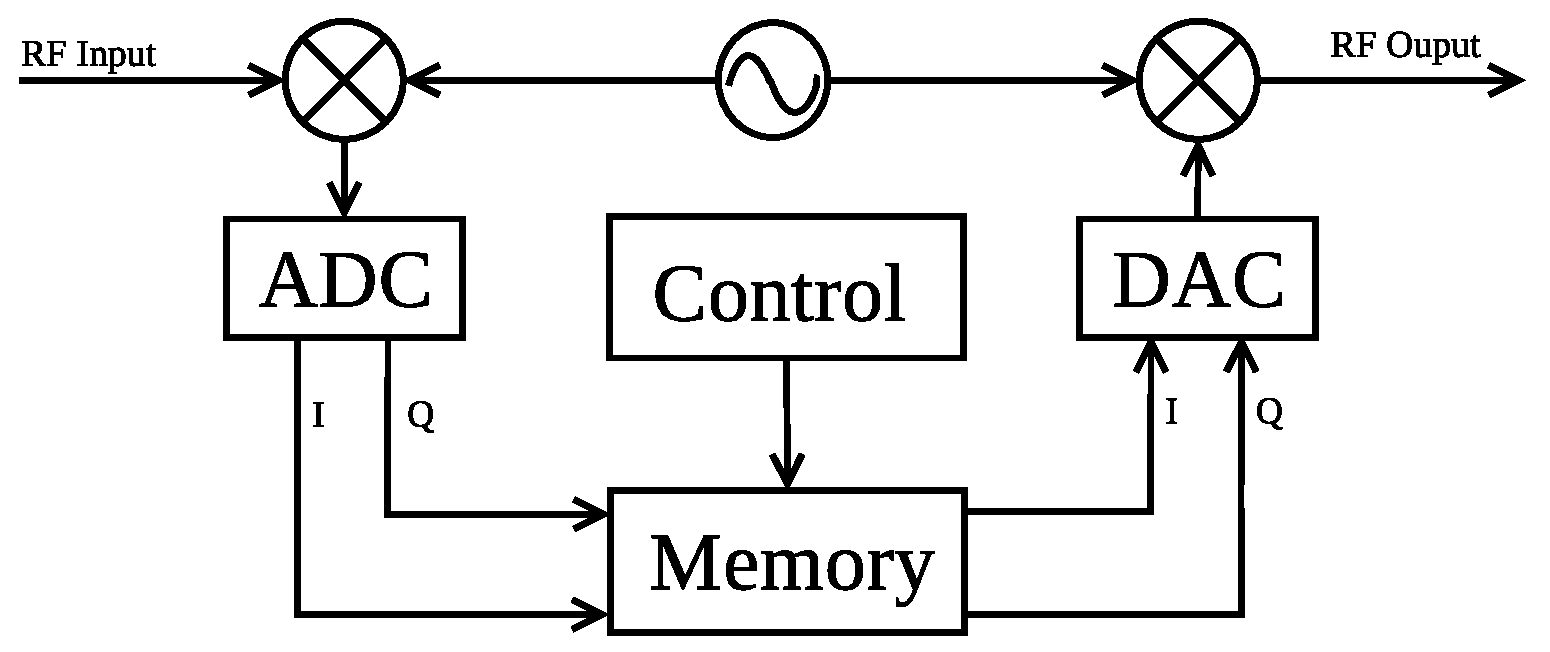
\includegraphics[width=0.8\linewidth]{img/DRFM_Intro}
		\caption{Illustration of DRFM System}
		\label{fig:DRFM_Intro}
	\end{figure}
		


